% gyrosope
% accelerometer
% seismometer
% perimeter security (fences)
% Fiber-optic hydrophones
% Fiber-optic bio-sensors \bibitem{chemsens}

najzaujimavejsie casti kodu
dat do prilohy


popisat websocket
asyncio a porovnat s multiprocessmy a multithreading


\chapter{Theoretical introduction}


Light has revolutionized data transmission and made high data rates possible using optical fibers and laser diodes. Apart from the intended usage, data transmission lines made from optical fiber have a new use case in sensing. The optical fiber can be used to measure useful external properties thanks to detection of different light scattering effects of the interaction between the light and the fiber.

In this work we will discuss fiber optics, optical reflectometry, distributed sensing, different light scattering effects happening in the fiber.

\cite{dasKislov}



\cite{DVSShanFu}


\section{Fiber-optic sensing}

Fiber-optic sensing uses optical fibers to measure different external properties. This works by 

is useful in environments that would be dangerous or harsh otherwise. Environments such as flammable, explosive, high voltage or environments that would create electromagnetic noise in other kinds of sensors. It uses fiber-optic cables as sensors.


For usesFiber optic cables used for 
% Advantages wire is stable, can be submerged in chemicals \bibitem{chemsens}



There are two types of optical fiber sensors:
\begin{enumerate}
    \item Point - These sensors measure only at the location of the transducer
    \item Distributed - The sensing element is the optical wire and can measure at many points along the optical wire. One of the great benefits of this approach is the possibility of using existing telecommunication infrastructure to build the sensing network.
\end{enumerate}

\subsection{Perimeter security}

% In this subsection we will discuss different fiber optic sensors that were used for perimeter protection. 
In the early 2000s perimeter protection using fiber optics was based on breaking or cutting the fiber which then triggered an alarm. This is good enough for one time use, because after the wire is broken there is no choice but to replace or repair the wire. This system can not tell the location when using single wire. Newer systems used \textit{Sagnac effect}, which uses Sagnac interferometer and a closed loop made of fiber optic wires for example 3x3\footnote{three by three} wire system. Sagnac interferometer detects changes in phase of light and thanks to signal processing and calculating the the time difference between amplitudes the position of intruder is calculated. Such interferometer has conversion unit from optical to electric signal. The electric signal is then sampled using fast A/D converter with high sampling rates. The accuracy of such system is 20-50 meters which is more than sufficient for perimeter protection\cite{perimeterpolsko}. 

\begin{figure}
    \centering
    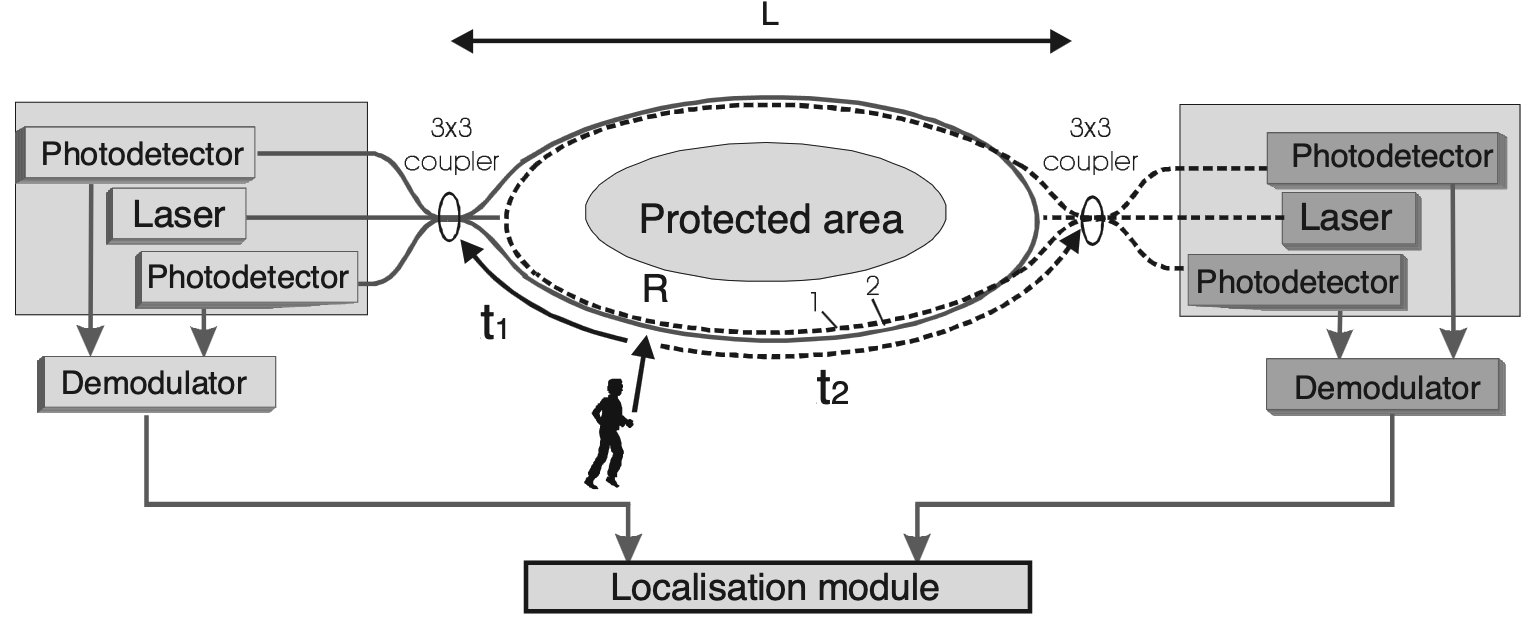
\includegraphics[width=\linewidth]{obrazky/sagnac_interrogator.png}
    \caption{3x3 system for perimeter protection using two Sagnac interferometers\cite{perimeterpolsko}}
    \label{fig:sagnac}
\end{figure}

Nowadays thanks to research and advancements in technology new devices based on DAS systems are used. These systems use scattering effects that happen in the fiber during the passage of photons through the medium that the fiber is made of. These effects are then analyzed at the source of light. The light bounces from imperfections in the fiber and is propagated backwards as scattering (\textit{backscattering}). There is nothing special happening when the fiber is not moving but when the fiber is affected in any way for example by vibrations of an intruder or just by voice alone the backscattering changes. These changes can be then analyzed, categorized as an intrusion.


\section{Optical fibers}

Optical sensing uses existing fiber optic transmission lines it is important to account for different kinds of optical fibers, materials, production methods.

Optical fibers consist of three main elements \textit{core}, \textit{cladding} and \textit{coating}. Materials from which core and cladding are made are plastic or glass $Si_2O_3$. Dopants, such as $GeO_2$, $P_2O_5$, $B_2O_3$, can be added to all-glass fibers to adjust refractive index. The core usually has higher refractive index than cladding by about \qty{1}{\si{\percent}}. Lowering refractive index can be done by doping fluorine, which is done in the core when the refracting index is too high and needs to be lowered\footnote{https://www.rp-photonics.com/fiber\_core.html}. The radius of core ranges from \qty{3.7}{\si{\micro}\meter} to \qty{200}{\micro\meter} and radius of cladding is up-to \qty{140}{\si{\micro}\meter}\cite{}.

Plastic optics uses organic material in the form of polymers - chains. Materials used are acrylic, poly-carbonate, polystyrene or liquid silicone. The core of plastic fiber has popular diameter of \qty{980}{\si{\micro}\meter}.

Although the purpose of coating is simply protective without it the fiber would be very fragile. It is usually without special color but can be painted to ease identification of individual fibers. There are multiple layers of coating at least primary and secondary. Primary is softer to allow bending of the fiber. Secondary is harder to protect inner layers. Materials such as acrylate, silicone, polyimid or carbon are used depending on application of the optical fiber. for example. For example acrylate has limited temperature resistance, in this case silicone is better as it is heat resistant up to \qty{200}{\celsius}\cite{cabling}. For more extreme applications Polyimid is used as it can withstand temperatures up to \qty{350}{\celsius} and it is also resistant to chemicals and abrasion\cite{cabling}.

\subsection{Fiber modality}

Optical fibers can have different kinds of modality depending on manufacturing processes, design decisions and it is a desired effect. We differentiate multimode and single-mode fiber optic cables. 

Multimode optical fibers have much larger core diameter compared to the diameter of cladding. This enables 


Single mode fibers have single propagation mode  per polarization fir a given wavelength. They have very small core diameter, only few micrometers, relative to the cladding diameter. Since they use only single mode there is no inter-modal dispersion\footnote{https://www.rp-photonics.com/single\_mode\_fibers.html}






Zamedzeny odposluch - po

When light travels from one medium into another reflection and refraction occurs. ReflectionFresnel reflection 




\section{Light scattering effects}

Light precisely photons travelling through a medium - atmosphere, glasses, glass optical fiber or any other medium can bounce from what is called \textit{scattering centers} in the medium. \textit{scattering centers} can be any non-unifomities in the medium such as vacancy defects (missing atoms in otherwise uniform structure), foreign particles, bubbles, trapped gas molecules, fractures, micro-cracks, changes in refractive index, density fluctuations, manufacturing imperfections and others\cite{scatteringcenterbook}.



\label{miesctt}
\subsection{Mie scattering}

Mie scattering is optical phenomenon happening when light is bouncing from \textit{scattering centers}\footnote{} bigger than the wavelength of the light

 amplitudes are stronger for forward scattering in Mie scattering


\subsection{Rayleigh scattering}

Rayleigh scattering is an optical phenomenon named after British physicist Lord Rayleigh. Light is scattered from scattering centers much smaller that the wavelength of the light for example individual molecules or atoms. This is opposite to Mie scattering \ref{miesctt}, where light is scattering from larger scattering centers. Difference is that amplitudes are stronger for forward scattering in Mie scattering\footnote{https://www.rp-photonics.com/rayleigh\_scattering.html}. Compared to other scattering processes Rayleigh is \textit{linear} scattering process whereas \textit{Raman} and \textit{Brillouin} scatterings are \textit{nonlinear}\footnote{Nonlinear light effects occur when the output intensity does not increase proportionally to the input intensity; for example doubling the optical input intensities does not result in double the output intensity. These nonlinear effects tend to weaken significantly at low optical intensities.}.

Only a small portion of the backscattered light gets back to the source. Most of it leaves the fiber on the sides. 


Not all scattering centers when solidified in a medium cause Rayleigh scattering. At a wavelength of about 0.95 μm (microns) glass optical fibers have a high attenuation band, which is caused by scattering and absorption by hydroxide ions\cite{scatteringcenterbook}. Silica glass is an amorphous material and as such has random density fluctuations due to its irregular microscopic structure. This can be limited by an annealing process but can not be removed completely\footnote{https://www.rp-photonics.com/rayleigh\_scattering.html}.






\subsection{Raman scattering}

The effect photons have when interacting with the crystal lattice of glass is called \textit{Raman scattering}. A transparent optical medium, such as glass, has a crystal lattice. The lattice is naturally vibrating and causing a delayed nonlinear response to the light passing through it. The photon travelling through the medium experiences a loss in energy due to interactions with the medium. This is also called \textit{inelastic scattering}. 

% The losses happen as vibration energy is exchanged between what are called \textit{phonos}. 

Raman scattering can be measured when sending two light waves with different wavelengths through the optical medium. The  signal with longer wavelength experiences optical amplification in expense of the one with shorter wavelength. This is used in Raman lasers, Raman amplifiers or Raman spectroscopy\footnote{https://www.rp-photonics.com/raman\_scattering.html}.

\subsection{Brillouin scattering}


https://www.rp-photonics.com/brillouin\_scattering.html
Brillouin scattering is used in Brillouin spectroscopy
\cite{bhundred}

\section{Optical reflectometry}

Optical reflectometry is used for measuring of properties of optical cables; it is capable of detecting defects, joints, breaks, or other damage and their location on the wire. It is the basis for \ac{generalotdr} or \ac{ofdr} and other optical sensors such as \ac{das}. A~pulse of light is sent from the source, such as a light-emitting diode (LED) or a laser diode (LD). The light travels from the source through the optical fiber in pulses and is reflected from the other side of the wire, through connections, breaks, damage, or imperfections in the material. All of these create some backscattering toward the light source. Rayleigh, Brillouin, and Raman scattering are all different kinds of scattering happening in the fiber \cite{progress}. 

\subsection{OTDR}

\ac{otdr} is the most widely used method. When a strain is applied to the fiber, it causes phase-shift changes in the light signal. Provides high sensitivity, resolution, and high sampling rates in the frequency range between hertz and kilohertz. \ac{otdr} has limitations in measuring slowly changing effects and noise components.

\subsection{(\acs{otdr})}   %\acl{otdr} 

\acl{otdr} 

https://www.flukenetworks.com/expertise/learn-about/otdr


\subsection{OFDR}

\ac{ofdr} analyzes interference of signal between the initial signal and the backscattered signal but focuses on the frequency scan. It requires a highly tunable laser diode as a~source of light. The signal given by \ac{ofdr} contains frequency information that can be processed with the Fourier transformation, and the output would be the position of the reflective elements along the fiber length. There are also other methods to measure light properties such as \textit{C-OFDR} - coherent version of OFDR using light with the frequency with linear dependency but having problems with high noise levels, and \textit{DSS} - Mandelstam-Brillouin \cite{kislov_das_newparadigm}.


\section{Distributed Sensing}

Distributed sensing (in general) is technology using optical fiber as an array of sensors. It was started from the field of optical reflectometry. With use of distributed virtual sensors along the fiber that are not real devices rather a clever way of measuring differences in the light signal properties such as changes in phase. It can measure tension, compression, temperature, vibrations other strain that is having an impact on the fiber and consequently the light passing through it\cite{dasKislov}.

We distinguish multiple distributed sensing systems depending on what is measured:
\begin{itemize}
    \item \ac{das} - recording sound
    \item \ac{dvs} - vibration detection
    \item \ac{dss} - twisting, pulling, bending
    \item \ac{dts} - temperature measurements
\end{itemize}

\subsection{Distributed Acoustic Sensing}

Implementation of \ac{das} system is usually done by \ac{generalotdr}, \ac{ofdr}, or analysis of other light properties such as polarization and backscatter correlation. \ac{das} allows the measurement on thousands of points on an optical wire without the need to cut the wire or have multiple sensors distributed along the wire. The measurement mechanism is based on optical reflectometry the same as in DTS (distributed temperature sensing), which is a variant of \ac{generalotdr}. During measurement pulses of light are sent into the optical fiber. The fiber creates a light scattering (e. g. Rayleigh scattering) in the glass that travels back to the sensing unit (on the same side as the light source), which can be interpreted on the basis of the time of arrival as position on the wire. Backscattering light from the optical fiber segment is detected at the light source and has changes in amplitude or phase, which means that the fiber wire segment is externally affected in some way. \ac{das} is used in a wide range of applications, from locating seismic activity, locating trains along the train tracks, as a~gyroscope or an accelerometer or even as a~microphone \cite{WangYu2017RDVM}, \cite{kislov_das_newparadigm}.

\ac{das} uses optical fiber as many sensors along its length. The fiber is  capable of detecting vibrations along it can also detect acoustic properties as they are also vibrations but of sound. These sensors allow for the measurement of acoustic properties such as frequency, amplitude, and phase \cite{WangYu2017RDVM}. 


% \subsection{Raleigh scattering}

% For a given optical frequency, sensors based on Raleigh scattering can detect the intensity, phase, and polarization of light.   
% %TODO

\subsection{iDAS}

The distributed acoustic sensor is a~new addition to distributed optical fiber sensors used in the energy industry and can be used in many applications, for example, in detecting seismic activity. iDAS (intelligent distributed acoustic sensor) is one type of DAS sensor. One of the applications of this sensor is to record an acoustic signal. To determine the signal fidelity, a certain part of the wire is subjected to a known signal, e.g. sine wave. A measurement is made, and the result is compared with the existing recording device. The result suggests that iDAS has very good signal properties. The measured signal shows that almost no measurable crosstalk is exhibited between the two sensing channels on the wire.

The maximum sampling rate can be calculated from the speed of light that travels in glass at a speed of about \qty{200000}{\km/\s} which corresponds to approximately \qty{10}{\kHz} for \qty{10}{\km} long wire \cite{WangYu2017RDVM}.

% 10 kHz == 10 km, 1 kHz == 100 km [doplnit vzorcek]

\begin{itemize}
    \item Acoustic bandwidth
    \item Dynamic range - \qty{120}{\dB} as reported in \cite{dasseismic}
    \item Spatial resolution - about \qty{1}{\m} to \qty{10}{\m}, but up to \qty{25}{\cm} is possible
    \item Measurement range - The fiber length can be anywhere from a few hundred meters to more than \qty{100}{\km}.
\end{itemize}



\section{OptaSense ODH-F}

Data used in this project were obtained from \textit{OptaSense ODHF Distributed Acoustic Sensing Interrogator}\footnote{\url{https://www.optasense.com/technology/odhf/}}(Interrogator). This device is capable of monitoring optical fiber up to \qty{50}{\km} long (in qualitative mode). It is used for in-well flow monitoring, pipeline integrity management, and border security. OptaSense comes with \textit{DxS Visualization Software} which is capable of analyzing and processing output data from the unit. It can show the signal spectrum in a waterfall graph and create analysis, process the signal using \ac{fft}, and extract data to \verb|.wav| format. It has the limitation that it can only run in the Windows ecosystem and is proprietary software, so scientists cannot really change how they work with the data or how it is displayed.


\subsection{HDF5 file format}

The data captured by the Optasense Interrogator is collected in \ac{hdf} and saved into a file with \textit{.h5} suffix. \ac{hdf} creates a model for managing and storing data. The HDF Group\footnote{\url{https://www.hdfgroup.org/}} is the maintainer of the format and its coresponding software package. Specifically, the \ac{hdf} format is used to store data, but it is only one of the three parts that make up the full \ac{hdf} model. Parts of the \ac{hdf} model are:

\begin{itemize}
    \item File format - files ending with .h5
    \item Data model - specifies the building blocks of the \ac{hdf} file format
    \item Software - libraries, tools, APIs
\end{itemize}

\bigskip

\ac{hdf} data model has a folder-like organization, where the folders are called \textit{groups}. This model specifies the format in which the data are stored in the form of \ac{adm}, which specifies the organization of the data and the types of data. Every \ac{hdf} file has to have a~root group \textit{``/''}. Working with groups is very similar to directories on Linux systems; see Section \ref{dir:filestructure}. Each group can have \textit{datasets} that contain raw data, attributes, data types, and other objects. \ac{hdf} file can also specify links to other libraries and tools such as compression and filtering.

\bigskip
HSDF5 dataset has connections with other HDF5 objects:

\begin{itemize}
    \item \textbf{attributes} - named data object containing the name and the value
    \item \textbf{datatypes}:
    \begin{itemize}
        \item Atomic datatypes - time, string, integer, float.
        \item Composite datatypes - array, enumeration, compound, variable length.
    \end{itemize}
    \item \textbf{data} - data itself, for example, the result of measurement.
    \item \textbf{dataspace} - the shape of the data.
\end{itemize}


\begin{figure}
    \centering
    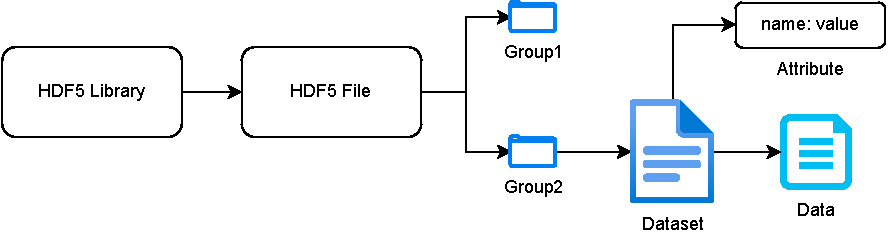
\includegraphics[width=\linewidth]{pdf/hdf5_file_structure.pdf}
    \caption{Basic HDF5 file structure}
    \label{fig:filestructure}
\end{figure}

\newpage %%%%%%%%%%%%%%%%%%%%%%%%%%%%%%%%%%%%%%%%%%%%%%%%%%%%%%%%%%%%%%%%%%%%%%%

\chapter{Implementation and software design}

\section{Program implementation of HDF5 to WAV}\label{lab:hdftowav}

The goal of this project is to create an application for reading data from the \ac{das} system and converting the data to the \verb|.wav| audio file format.

For the implementation of this application, the Python\footnote{\url{https://www.python.org/}} programming language was chosen. Python is a~great language for scientific use, data visualization, and graph plotting, which is the goal. The biggest advantage comes from the availability of scientific libraries. The opening of \verb |.h5| files is done with \verb|h5py| library\footnote{\url{https://www.h5py.org/}}. For working with dataset data types \verb|numpy|\footnote{\url{https://numpy.org/}} library is used. The function for interpolating arrays to a~certain range is also used \verb|interp|. Lastly, to convert the signal data to \verb|.wav| audio format \verb|scipy| library is used specifically \verb|io| module function \verb|wavfile|. To read all options and input arguments, the \verb|argparse| library is used\footnote{\url{https://docs.python.org/3/library/argparse.html}}.   

\subsection{Reading HDF5 file}\label{sec:readhdf}

The sample file recorded in the OptaSense ODH-F is in HDF5 file format. As \ac{hdf} files have a~user-defined structure on the application layer and in the binary form it is hard to say what is actually in the file. To better understand the contents of the \verb|.h5| file, \verb|h5dump| was performed and a conversion to JSON\footnote{\url{https://www.json.org/json-en.html}} was also performed by the \verb|h5tojson| program\footnote{\url{https://hdf5-json.readthedocs.io/en/latest/tools/h5json.html}}. The JSON file is quite large in size - the original HDF5 file is only \qty{52,7}{MB} and the JSON file is \qty{946,6}{MB}. The dump text file is half the size and provides the same information, but the datasets are harder to understand, but the whole file is only half the size of the JSON file at ``only'' \qty{420}{MB}. The JSON format is much easier to read. The structure of the file is divided into 3 parts:

\begin{itemize}
    \item \textit{apiVersion} - 1.1.1 version of API
    \item \textit{datasets} - Contain all the datasets organized by their UUID\footnote{Universally unique identifier} that are defined in the groups section. There is also an \textit{alias} that is in the format of a Unix-based system path, for example, \verb|"/Acquisition/Raw[0]/Custom/SampleCount"|. There are also other properties that define the shape and type of stored data. In this case, the properties are shown in the table \ref{tab:file_details}.
    \item \textit{groups} - Groups are named by a UUID. The group object has:
        \begin{itemize}
            \item \textit{alias} - Unix-like name; the first is root ``/'' group
            \item \textit{attributes} - define the type, name, and shape of the value of the attribute which is a string \verb|979bb2ac-99bf-4cb5-b410-5c16cd7872dc|
            \item \textit{links} - links to other groups that create a treelike structure. The link object contains the class of a link (e.g. H5L\_TYPE\_HARD for hard link), the \textit{collection} property telling that it is a group and the name of the group. The group object also contains other important metadata, such as measurement settings. All important details are given in the table \ref{tab:file_details}
        \end{itemize}
\end{itemize}

There is a~library for reading \ac{hdf} files using Python called \verb|h5py|. To read the contents of the file, a~function was created called \verb|get_dataset_path()| which recursively looks for all groups, according to their name provided by the \verb|.keys()| method, in the dataset. The result of this function is propagated through recursion and saved in Python \verb|set()| built-in type. The user can then choose which one is the right dataset to use because there is probably more than one dataset. The user can save the string and use it as an argument when calling the program. This saves time in searching for the contents of the file. 

This is the data structure of the DAS file from the OptaSense Interrogator:

\bigskip
DAS output file structure in \ac{hdf} format
{\small
%
\label{dir:filestructure}
\dirtree{%.
.1 /\DTcomment{root}.
.2 Acquisition\DTcomment{Recorded data}.
.3 Custom\DTcomment{Empty}.
.3 Raw[0]\DTcomment{HDF5 group (3 members)}.
.4 Custom\DTcomment{HDF5 group (1 members)}.
.5 SampleCount\DTcomment{HDF5 dataset, shape (332032,), type "<i8">}.
.4 RawData[0]\DTcomment{HDF5 dataset, shape (100, 332032), type "<i2">}.
.4 RawDataTime\DTcomment{HDF5 dataset, shape (332032,), type "<i8">}.
}
}
\bigskip

The type of explanation in \ref{dir:filestructure} is \verb|i8|, which is \verb|numberpy.int64|. \verb|SampleCount| contains numbering of all samples, \verb|RawDataTime| contains time, and \verb|RawData[0]| contains useful sensor data that we need to read in the next steps; see \ref{sec:data_processing}. More details are provided in Table \ref{tab:file_details}.

All important HDF5 attributes are shown in the table \ref{tab:file_details}, it contains metadata information about the datasets, data dimensions, number of channels, kinds of filters used, time information, length of pulses, laser wavelength, and more. Some properties can be derived from those in the table. The capture duration can be calculated from the start and end of the capture, which is \qty{10,376}{\second}.

\subsection{Data processing} \label{sec:data_processing}

The useful data have 100 channels with \textit{N} samples, in this example \qty{332032}{samples} saved in \verb|/Acquisition/Raw[0]/RawData[0]|, see the file structure in \ref{dir:filestructure}. The function \verb|scipy.io.wavfile.write()| is used to save samples to a file and the data need some more processing before the function can be called. After the data are read from the file, it is saved into \verb|samples| variable of type \verb|numpy.array| it is then processed in 4 steps as preparation for saving into \verb|.wav| file. The steps are:

\begin{enumerate}
    \item \textbf{Channel selection} - only channel one can be selected.
    \item \textbf{Data interpolation} - The original data have a bad value range from -24838 to -30758, triggering an exception when writing the data into a \verb|.wav| file. The \verb|numpy.interp()|\footnote{\url{https://numpy.org/doc/stable/reference/generated/numpy.interp.html}} function interpolates the data into the range of the maximum and minimum values specified in this case by the \qty{16}{bit} PCM\footnote{Pulse Code Modulation}, which can be written to WAV file by \verb|wavfile| module.
    \item \textbf{Resampling} - as the data are recorded at a certain sampling frequency, in this case, \qty{10}{\kHz}, resampling by the function \verb|scipy.signal.resample() |\footnote{\url{https://docs.scipy.org/doc/scipy/reference/generated/scipy.signal.resample.html}} is necessary. The right number of samples is calculated by the formula \ref{formula:sampling}.
    \item \textbf{Retyping} - the resampled data need to be in the correct format and since the interpolation was done in the range of \verb|int16| the output type of choice is the same \verb|samples.astype(np.int16)|.
\end{enumerate}

\begin{equation}
    \label{formula:sampling}
    numSamples = \frac{44100}{fs.len(samples)}
\end{equation}


\begin{table}[]
    \centering
    \begin{tabular}{|c|c|c|c|}
    \hline
    \textbf{Data type} & \textbf{Minimum value} & \textbf{Maximum value} & \textbf{WAV format} \\
    \hline
    float32 & -1.0 & +1.0 & 32-bit floating-point \\ \hline
    int32 & -2147483648 & +2147483647 & 32-bit PCM \\ \hline
    int16 & -32768 & +32767 & 16-bit PCM \\ \hline
    uint8 & 0 & 255 & 8-bit PCM \\
    \hline
    \end{tabular}
    \caption{WAV compatible types}
    \label{tab:my_label}
\end{table}




\newpage

\section{Software design}


There are many ways to implement data visualization, but it is hard to choose the right solution, the right programming language, or a framework, so this chapter first provides information on what this application should do. Second, it provides a study of the existing OptaSense software and other solutions accessible from the internet. Lastly, it explains the software design decisions for the implementation of this data visualization.

\subsection{Usecases}\label{lab:usecases}

The task is to fulfill the requirements and basic usage as can be seen in the use case figure \ref{fig:usecase}. They need to see and view what is happening in their perimeter on their screen. For this purpose, the best data visualization is a waterfall graph, similar to a spectrogram, displayed as the main element. It should have an editable color map to change the sensitivity. The waterfall view should be a fully animated waterfall graph and ideally display real-time data on the screen, similar to the OS6 system; see Section \ref{sec:ossix}. In addition, the user should perform selection and zoom on the waterfall graph. The user should be able to edit properties of the graph, like changing the data range and choosing the channels he or she wants to see. The user should be able to export the data to a WAV file by clicking a button and then viewing and playing the audio file. There should also be a waveform display available to show the playing data.

\begin{figure}[h]
    \centering
    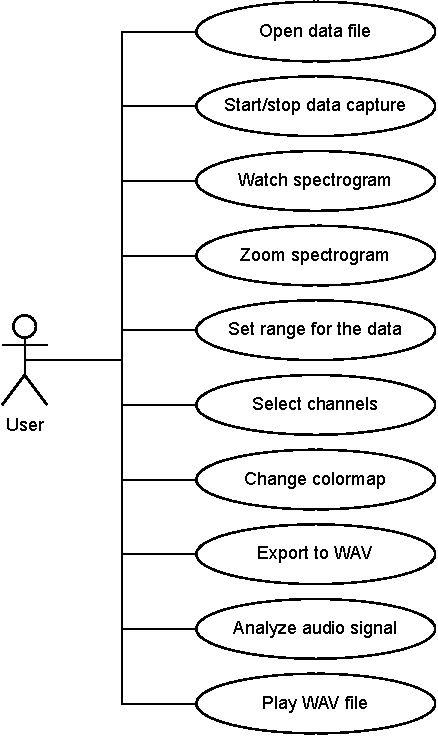
\includegraphics{pdf/usecase.drawio.pdf}
    \caption{Application usecases}
    \label{fig:usecase}
\end{figure}

\subsection{Application requirements}

From the use cases in Section \ref{lab:usecases} it is understandable that the application should have certain features. Apart from the given use cases, there are other important requirements:

\begin{itemize}
    \item Support for real-time data plotting - graph updates or animation; fetching the data online from the OptaSense Interrogator and displaying it in real-time
    \item Multiplatform - the application should run on any device and still support all features
    \item Data processing - subsampling data to save data throughput
    \item Plot editing and animation - changing plot properties
    \item Reading offline data - possibility to read local files or upload files into the application
    % \item 
\end{itemize}

% There is the option to create an application running on the operating system

\begin{figure}[h]
    \centering
    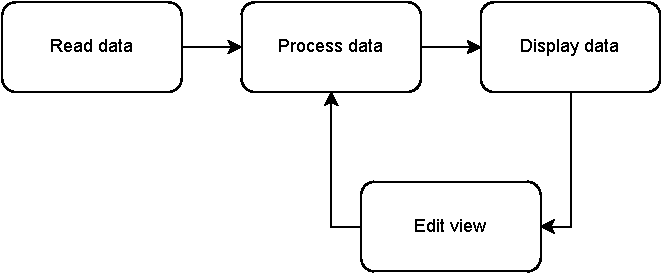
\includegraphics{pdf/simple_application.drawio.pdf}
    \caption{Data flow in the application - reading the data then processing the data and displaying it (optionally) edit the view}
    \label{fig:dataflow}
\end{figure}

It is necessary to choose the right programming tools to satisfy all features. The right way to find the right solution in programming is to \textit{divide and conquer}. This means finding all the pieces that will make the application. First, there must be an idea of what will happen with the data. Firstly, it has to be read, processed, and then displayed, the optional step is to edit the data or change the view; this data flow can be seen in Figure \ref{fig:dataflow}. 

% Multiplatform requirement removes many options - like creating a simple GUI application, as creating a multiplatform high-performance application is quite a feat and is beyond this project. So the result is making a web site and display  there is one solution either using 

From the data flow application, an overview can be made for a web application, as can be seen in Figure \ref{fig:app_overview}. The overview illustrates what parts the application will have. The back-end or server application will be responsible for reading HDF5 files and processing data. It will provide some form of interface or API for the client application to fetch\footnote{\url{https://developer.mozilla.org/en-US/docs/Web/API/Fetch\_API}} the data. On the client side, the client has to be able to create visualizations of the data and provide a user interface to change application properties.

\begin{figure}
    \centering
    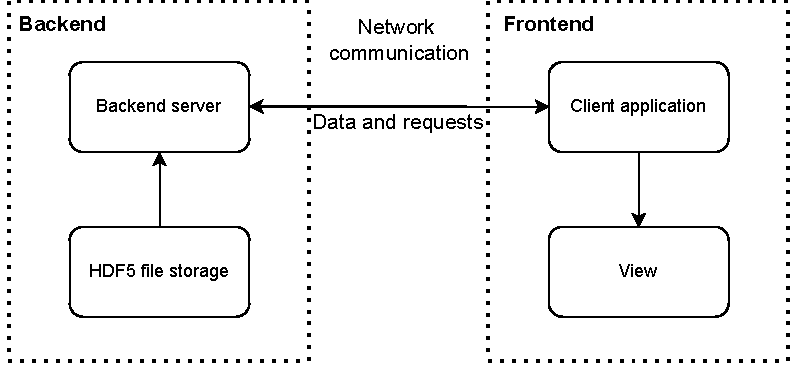
\includegraphics{pdf/appstack_general.drawio.pdf}
    \caption{Application overview. The server reads the data from the data storage and sends it to the client application, where it is shown to the user}
    \label{fig:app_overview}
\end{figure}

\section{Existing technology for data visualization}

This section focuses on data processing and visualization using existing software for visualizing scientific data. First is OptaSense OS6 software which is a purpose-made solution for OptaSense devices. Next is the h5web library, written in React, which creates a web page for visualizing the content of HDF5 files.

\subsection{OptaSense OS6}\label{sec:ossix}

The OptaSense company provides visualization software for their devices called OptaSense OS6\footnote{\url{https://www.optasense.com/technology/os/}}. It runs only on the Windows operating system. OS6 provides features for monitoring certain areas or land, for example, a compound or an industrial building. This product is tailor-made for OptaSense devices by the OptaSense company. This system has only one window for everything. The main view is the monitored area; the background picture is the aerial view of the whole monitored space, as can be seen in the picture \ref{fig:ossix}. The user can open the sidebar on the right side. The sidebar provides multiple different options:

\begin{itemize}
    \item \textbf{Spectrogram} - Raw data visualization.
    \item \textbf{Alerts} - When an action is detected along the wire, it is logged.
    \item \textbf{Notifications} -  Notifications about system state.
    \item \textbf{System status} - Overview of all OptaSense units and their state.
\end{itemize}

There is also a feature that takes raw data from interrogator units and processes them using machine learning. In this way, different actions are detected and categorized into different types of alerts, such as walking, driving cars, etc. In addition, the user can see the activities that were detected and triggered in the area overview with live monitoring and a timeline at the top of the screen. To easily look at different locations or start a new view, there is a feature \textit{type to search} that lets the user start a search by typing into the view. For example, the user starts writing ``water...'' as a waterfall, and the program will look for this feature and open the waterfall visualization window. OS6 saves all detected activities, which can be shown in the \textit{Historic timeline} window, which shows all alerts that occurred during a specified time range. The animations look very nice, although some of them look a bit choppy mostly when showing activities on top of the waterfall view. 

Anyway, it is proof that it is possible to create a real-time data visualization from the DAS system. It lacks one important step, which is the ability to be used not only on Windows machines and to be truly multiplatform.

\begin{figure}[]
    \centering
    \includegraphics[width=\linewidth]{obrazky/OSsix.png}
    \caption{OptaSense OS6 visualization software \cite{ytossix}}
    \label{fig:ossix}
\end{figure}

\subsection{h5web}

The \verb|h5web|\footnote{\url{https://h5web.panosc.eu/}} library is a set of components written in React\footnote{React is a JavaScript library used to create interactive user interface \url{https://reactjs.org/}}. H5web uses existing HDF5 libraries, such as h5wasm (reading HDF5 files in the browser) and h5grove (server for accessing HDF5 files). It displays the contents of HDF5 file, as well as shows different graphs according to the input from the user. From the presentation of the library by its developer it is safe to say that although it provides the necessary equipment for opening HDF5 files elegantly and provides advanced graphing techniques it lacks the ability to receive the data and display them in real-time. For this purpose, the library would need to add support by creating a new React component capable of such behavior, but it is possible.

\subsection{Backend}

The purpose of the backend part of the application is to read, process, and send the data to the client part of the application, as can be seen in Figure \ref{fig:app_overview}. Reading the HDF5 data is done as explained in Section \ref{sec:readhdf}.

\subsubsection{REST servers}

There is a wide range of REST server implementations; HDF Group provides documentation for its RESTful API\footnote{\url{https://support.hdfgroup.org/pubs/papers/RESTful\_HDF5.pdf}}. They have prepared a few RESTful server implementations for their data format. There are many more implementations of REST servers, such as the Python Simple HTTP server. Here is a list of some possible implementations \cite{hdfrest}:

\begin{itemize}
    \item \emph{h5serv} - REST-based service to access HDF5 data written in Python (HDF5 Group).
    \item \emph{HSDS} (Highly Scalable Data Service)\footnote{\url{https://github.com/HDFGroup/hsds}} - Python implementation of the REST-based service to access HDF5 data stores. Data can be stored in the POSIX file system or using object-based storage such as AWS S3. It can run in a Docker as a single machine or on a Kubernetes cluster.
    \item \emph{hdf-rest-api}\footnote{https://github.com/HDFGroup/hdf-rest-api} - is HDF5 REST API that provides CRUD support (create, read, update, and delete) for all HDF5 objects.
    \item \emph{h5grove} - Backend service written in Python providing access to HDF5 file content.
    \item \emph{http.server} - Python implementation of a simple HTTP server. However, this is better used only for testing purposes when accessing local files.
\end{itemize}

\subsubsection{WebSockets}

WebSockets (or WebSocket API) enable two-way communication over TCP. It was standardized by IEFT in RFC6455. WebSocket protocol is supported by all modern browsers. The communication starts with an HTTP-compatible handshake, so only one socket can be used to communicate with the server. There are also other header types available for different uses. The server responds with an HTTP Upgrade, the connection is established, and bidirectional communication can begin. Communication closes when either side decides to close the connection and starts closing the handshake. The other side responds with a \textit{Close frame} message and the connection is closed. The protocol is trying to be frame-based as is HTTP but also frame-based as little as possible, just to make sure that it can use the HTTP interface for communication; otherwise it tries to be as minimalist as possible. The authors of the WebSocket protocol wanted it to be low-level and as close to TCP as possible \cite{websock}. WebSockets have an implementation in the Python programming language called \verb|websockets|\footnote{https://pypi.org/project/websockets/}.

\begin{figure}[h]
    \centering
    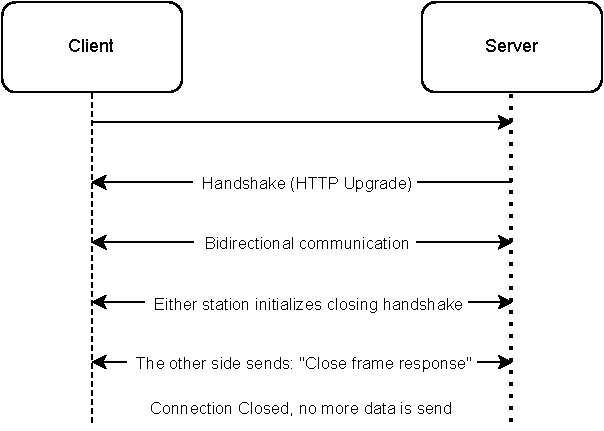
\includegraphics{pdf/websocket.drawio.pdf}
    \caption{WebSocket handshake, communication, and connection close diagram.}
    \label{fig:websocket}
\end{figure}

% \subsubsection{Processing data}\label{lab:processingdata}

% The data read from the file is in 

% %TODO







\subsection{Frontend}

% \subsubsection{WebGL}

% WebGL is a cross-platform web standard for 3D graphics API based on OpneGL, that is rendering into HTML \verb|<canvas>| element. It supports 
% https://github.com/bastibe/WebGL-Spectrogram


\subsubsection{Svelte}

Svelte is a component framework written in JavaScript, using a new approach to building web applications. Instead of looking for differences in virtual DOMs as React does, which is done in the browser and consumes quite a lot of resources, Svelte does everything at the compilation stage. The output of the compilation is a JavaScript file \verb|bundle.js|, which contains all the necessary code to run the web application or better said, it manipulates the DOM directly. The result is a fast and reactive web page, it also saves resources, and the code can be run on small devices like handheld devices. Web development is also very enjoyable because compilation does not take long and the changes can be visible immediately. The structure of a Svelte component consists of three parts - JavaScript code tag \verb|<script>| a style tag \verb|<style>| and other HTML elements. 

Svelte does not provide more advanced features like page routing. For this purpose, the Svelte team created SvelteKit, which is a~framework for building web applications and allows page routing. Routing is folder-based - the developer creates routing by creating a folder and file structure.

\begin{verbatim}
src/routes/about/+page.svelte <=> /about
src/routes/about.svelte <=> /about
\end{verbatim}

Svelte has been changing and has become a Vite \footnote{\url{https://vitejs.dev}} plugin. Vite provides fast development experience by running a development server, in the case of Svelte - Hot Module Replacement (HMR)\footnote{\url{https://vitejs.dev/guide/features.html\#hot-module-replacement}}. This way, every change made during development can be immediately seen in the browser without reloading the page, which makes development much faster and more enjoyable. It is necessary to say that Svelte is still in development and although it is now at version 3 it is possible that it will change in the future. 

When fetching the data from the server, it is good practice to move this functionality to a Svelte Store. From a programming point of view, a store is an object with a \verb|subscribe()| function. An example of a WebSocket implementation in Svelte can be the Svelte component library \textit{svelte-websocket-store}\footnote{\url{https://github.com/arlac77/svelte-websocket-store}}.

\subsection{Real-time capabilities}

The data bandwidth (the amount of data necessary to be sent from the server side to the client side) of the application is the biggest factor. The OptaSense Interrogator can produce quite a lot of data, but if it is saved in an HDF5 file, as it is compressed it is quite small. As discussed in Section \ref{sec:readhdf}, a \qty{10}{\second} file produces around \qty{52}{MB} of data. When this data is transformed into text form, it has only \qty{420}{MB} and when transformed into JSON, it has \qty{946}{MB} as the data are read at  \qty{10}{kSPS}\footnote{\ac{sps}}. Data will be displayed on a display with standard resolution and cannot display \qty{10000}{\ac{sps}} on a small part of the display. Data processing is necessary for this purpose. 

% \subsubsection{Data processing}

% Data processing can be done on the server side or in the browser. As the browser will be busy redrawing waterfall visualization it is better to do data preprocessing on the server side. Server-side preprocessing will also save bandwidth as the data will be significantly filtered. 

% Sending data in the form of REST requests and responses can be possible but it is really useful only when sending a small HDF5 file as a whole not as a stream of data and although h5grove backend provides the ability to read sections of the data set for  The respective bandwidth would be \qty{}{}



% %TODO


 % The JSON file is quite large - the original HDF5 file is only \qty{52,7}{MB} and the JSON file is \qty{946,6}{MB}. The dump text file is half the size and provides the same information, but the datasets are harder to understand, but the whole file is only half the size of the JSON file at ``only'' \qty{420}{MB}. The JSON format is much easier to read. The structure of the file is divided into three parts:

\subsection{Software design for DAS data visualization}

As we discussed in Section \ref{sec:ossix}, it is possible to create such software to display the data in real time. The application was a native Windows application, and the requirement for this application was to be able to run on multiple platforms. The chosen platform is the Python backend, opening files, processing the data, and sending the data into the client application using Svelte. The backend will process the data as explained in \ref{lab:processingdata}. The waterfall graph will be an HTML Canvas element that displays the data in real-time, redrawing itself as the data arrive at the browser. For ease of displaying the data in Canvas, D3.js will be used. D3 will, for example, apply a color map to the correct scale according to the data. The user interface written in Svelte will also have inputs to change the properties of the visualization so that the user can select specific channels from the data, choose subsampling effect properties, cutting the frequency range. The ability to export the data to a WAV file will also be implemented the same way as done in Section \ref{lab:hdftowav}.

\begin{figure}
    \centering
    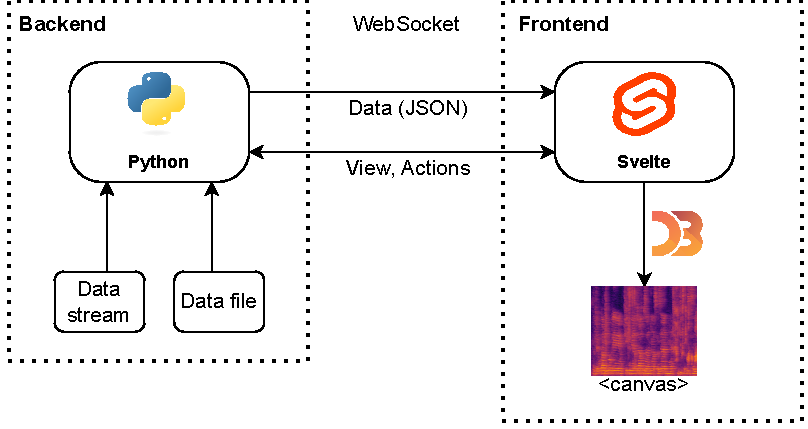
\includegraphics{obrazky/appstack.drawio.pdf}
    \caption{Application overview}
    \label{fig:app_overview}
\end{figure}

\subsection{Prototype}

This work aims to design an application to visualize HDF5 data acquired from the OptaSense Interrogator. For this purpose, Svelte was used mainly for its high performance, thanks to efficient code created at compilation. This is a prototype, so it is not a working application. It is only to show how this application will look in the end. The final version of the application will also use Svelte. The prototype uses Flowbite components\footnote{\url{https://flowbite-svelte.com/}} as they make it easy to create stylized web pages. The web page is divided into Svelte components. The main component is the waterfall graph on the left side of the screen and the control panel on the right side. Layout is done with svelte-layouts\footnote{\url{https://www.npmjs.com/package/svelte-layouts}} package. 

Uploading files into the browser using REST API was also tested. Python's \verb|http.server| was used as the backend. When fetching files into a browser from local storage using HTTP, it is necessary to allow Cross-Origin Resource Sharing (CORS) because browsers restrict this feature for security reasons. Some resources like CSS, Web Fonts, and WebGL textures have enabled CORS. For sending HDF5 files to the browser, a special HTTP header has to be added on the server side. Without this feature, the browser would throw an error into the JavaScript console.

\begin{figure}
    \centering
    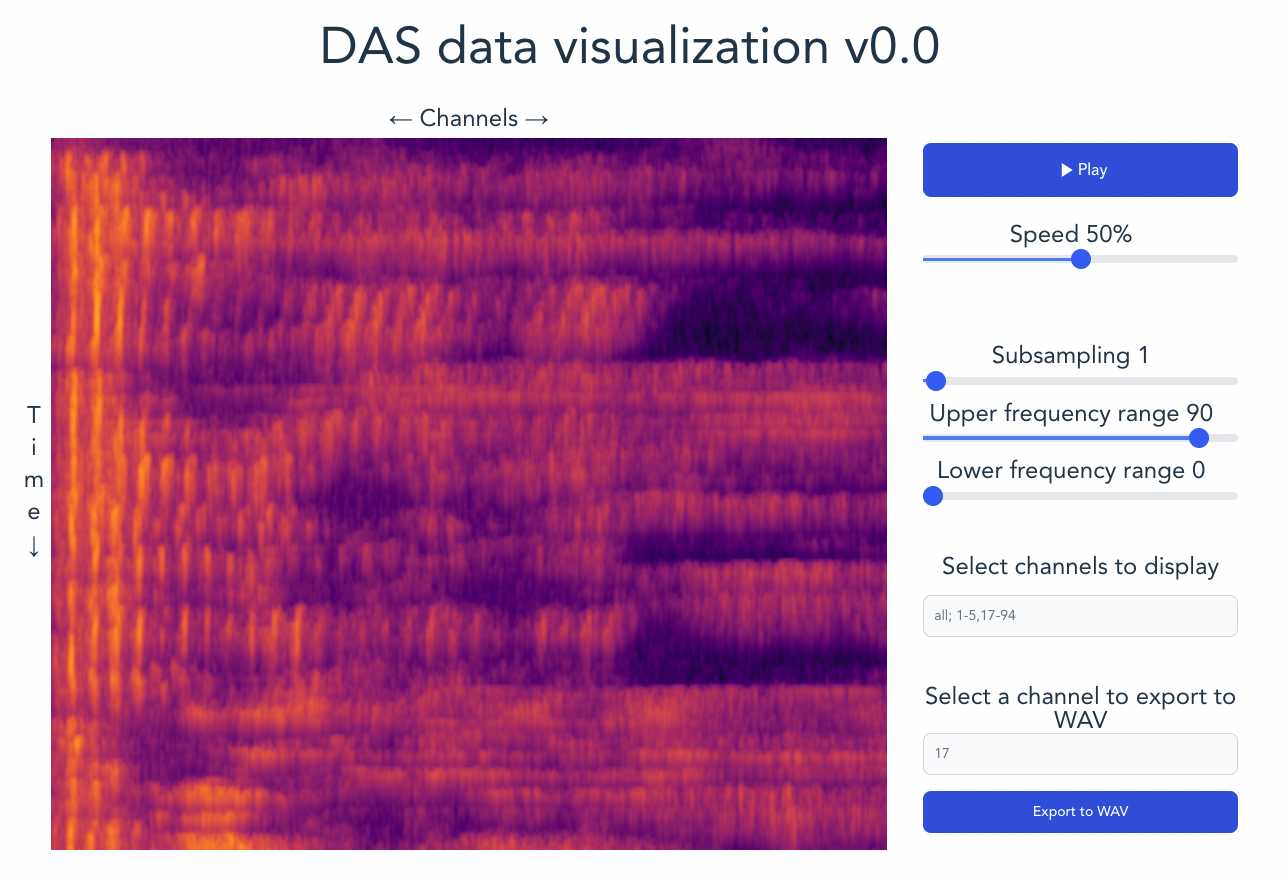
\includegraphics[width=\linewidth]{obrazky/svelte_prototype.png}
    \caption{Prototype of DAS visualization application}
    \label{fig:prototypesvelte}
\end{figure}






\chapter{Out of context}

\subsection{Colormaps}

Choosing a suitable colormap is crucial when displaying data to users. The colormap's purpose is to understandably represent the data so that it is easy for users to understand what is displayed in front of them. A colormap with equal steps between colors and steps in data is best perceived - this is called \textit{perceptually uniform colormap}. It was found that perception in change in color is best understood by human brain, rather than changes in hue. 

There are 4 basic colormap classes:

\begin{itemize}
    \item Sequential - used for ordering. Incremental changes in lightness and saturation of single color often with single hue
    \item Diverging - 
    \item Cyclic - 
    \item Qualitative - 
\end{itemize}
source https://matplotlib.org/stable/tutorials/colors/colormaps.html

https://github.com/d3/d3-scale-chromatic



\section{Svelte}

% A Svelte application consists of 


This subsection is based on Svelte documentation\cite{sveltedoc} and as Svelte is a new framework and its documentation is too simple for more complicated projects we also rely on what we learned from forums and videos.

\subsection{Components}

\subsection{Stores}

A \textit{store} is in general any Javascript object that correctly implements basic reactive methods \verb|.subscribe|,  \verb|.unsubscribe| and (optionally) \verb|.set| or \verb|update|. This allows basic reactive behaviour and makes it possible for Svelte components to then use this object to access and change its values. Stores are usually defined in \verb|.js| files and can be defined either as single store in a single file or multiple stores defined in a file. 

There are three predefined Svelte stores implemented in \verb|svelte/store| module. They are:

\begin{itemize}
    \item \verb|readable()| - creates a store whose value cannot be set from components it does not implement the \verb|set| or \verb|update| methods
    \item \verb|writable()| - creates a store which has values that can be set from the components. The writable store implements \verb|set| and \verb|update| methods. \verb|set| saves the the value given and saves it. \verb|update| method takes a callback that takes the existing store's value as its arguments and returns a new value to be set to the store.
    \item \verb|derived()| - creates a store whose value is dependent on other store. It runs initially when the first subscriber subscribes and whenever the dependency changes.
\end{itemize}


\section{HTML chart rendering}

For in browser rendering in there are two main options using HTML canvas rendering or using \ac{svg} elements. In this section we will discuss both, their advantages over each other and their drawbacks. In general Canvas rendering is better performing than \ac{svg} rendering. This is due to the fact that SVG is based on a \ac{dom} structure\footnote{text based structure defining objects that are displayed in the web page. https://developer.mozilla.org/en-US/docs/Web/API/Document\_Object\_Model/Introduction}. It is more suitable for large datasets and graphics heavy games and animations. 

\footnote{https://www.chartjs.org/docs/latest/\#canvas-rendering}


\subsection{Canvas graphics}

JavaScript makes drawing to the HTML \verb|<canvas>| element possible with the use of \textit{Canvas API} or \textit{WebGL API}. It can be used for rendering data visualizations, game graphics, real-time video processing and animation. Canvas API focuses on 2D graphics. Libraries using Canvas API that make rendering to canvas easier differ on the usecase - EaselJS (web game development), Konva.js (desktop and mobile applications), Chart.js and many more. Canvas rendering depends on the resolution of the screen. 

\verb|<canvas>| tag is used for drawing graphics. You can imagine canvas to be a rectangular area with the starting point at the top left corner with coordinates (0,0) and defined width and height. By default this area is transparent. When we want to draw to it we need to call functions from the Canvas API. They define basic shapes and primitives that can drawn on the canvas. Rectangles and paths are the only primitive shapes that can be drawn to \verb|<canvas>| element and more complex shapes can be drawn by combining these primitives\footnote{https://developer.mozilla.org/en-US/docs/Web/API/Canvas\_API/Tutorial/Drawing\_shapes}. Basic example of drawing to canvas can be seen in the code snippet \ref{lst:canvas.example}. Usually the functions define either certain shapes that are filled with color and are basically added to the canvas then there are "clearing" functions that remove what is displayed or creating transparent areas and lastly there are "stroke" functions that create lines. 

\begin{lstlisting}[frame=single,numbers=right,caption={An example implementation of drawing to canvas.},label=lst:canvas.example,basicstyle=\ttfamily\small, keywordstyle=\color{black}\bfseries\underbar,]
function draw() {
    // first we need reference to canvas element
    const canvas = document.getElementById("canvas");

    // next we need context to draw to
    const ctx = canvas.getContext("2d");

    /**** Drawing  ****/
    
    // drawing rectangle to canvas
    ctx.fillRect(10, 10, 100, 100);
}
\end{lstlisting}








These interactions are achievable in the canvas rendering but usually require "hacky" solutions like hidden canvas or like invisible layers. Having more than 1000 objects rendered on screen that can be selected can cause performance issues.

The biggest drawback of displaying data with canvas is its lack of interactivity with displayed elements and poor text rendering capabilities\footnote{https://www.w3schools.com/html/html5\_svg.asp}.

WebGL can draw 2D and 3D graphics to the canvas element.


\subsection{Drawing to canvas and animation}





Creating animations on canvas element is done by calling functions 
window.requestAnimationFrame()


\subsection{HTML SVG graphics}

\ac{svg} is an XML-based markup language developed by W3C\footnote{World Wide Web Consortium www.w3.org}. It describes 2D vector graphics in XML text files. SVG supports three types of graphic objects: vector shapes, bitmap images and text. The main advantage compared to bitmap graphics is that all the elements can be rendered at any size without the loss of quality. 

The description of graphics elements is the same way as the web page description written in HTML to the final web page. There are tags for different geometrical objects, for examples rectangle, ellipse, line and animations. Everything is defined in an XML text file which can be edited, searched or compressed\footnote{https://developer.mozilla.org/en-US/docs/Web/SVG}.

Data visualization using \ac{svg} graphics results in smooth and sharp visualizations. It also enables interactivity with each displayed object - selecting, hovering or zooming. Libraries for \ac{svg} manipulation are basically manipulating text, based on the data given. \ac{dthree} is a JavaScript libarary using HTML, SVG and CSS to visualize data. It can bind data to the HTML DOM and then apply data-driven transformations. \ac{dthree} allows developers to create custom visualizations as it is not a charting library rather a set of tools used for data visualization. It is also the base for other charting libraries that build on top of \ac{dthree}'f framework. They include Plotly's JavaScript implementation, C3.js\footnote{https://c3js.org/} or Britecharts\footnote{https://britecharts.github.io/britecharts/}.




Python implementacia - backend

Generator
websockets
